% Use the University of Michigan thesis class.
% options include report, thesis, debug, backref
\documentclass[thesis]{thesis-gwu}[2016/09/24]

\usepackage{lipsum}

% --------- FRONT MATTER PAGES ---------------------
% Title of the thesis
\title{Solving Nonlinear Equations of One Variable}

% Author name
\author{Shankar Kulumani}

% Previous degrees
\bsdepartment{Astronautical Engineering}
\bsschool{U.S. Air Force Academy}
\bsgrad{May 2009}

\msdepartment{Aeronautics and Astronautics}
\msschool{Purdue University}
\msgrad{December 2013}

% PhD degree commands
% Committee
\showcommitteepage
%\hidecommitteepage
\committee{ %
Taeyoung Lee, Associate Professor of Engineering and Applied Science,\\ 
Dissertation Director\\
Full Name, Title, \\
Dissertation Director/Co-Director/Committee Member
}

% Chair must be entered separately for formatting reasons.
\chair{Taeyoung Lee}
\chairtitle{Associate Professor of Mechanical and Aerospace Engineering}
% Department
\department{Mechanical and Aerospace Engineering}

\phdgrad{May 28, 2015}
\defensedate{May 28, 2015}
% Year of completion for copyright page and perhaps other places
\year=2015 

% Frontispiece
% delete to not print
\frontispiece{\includegraphics[width=4in]{./figures/frontispiece.pdf}}

% Copyright page
%\hidecopyright
\showcopyright
%\copyrightholder{Someone else}

% Default style for front pages
\frontpagestyle{3}

% Dedication
\dedication[8]{ %
\textit{to Christine}
}

% Acknowledgments
\acknowledgments[3]{ %
This template is a fork of the great work done by Derek Dalle~\url{http://www-personal.umich.edu/~dalle/codes/thesis-umich/}.
None of this would be possible without the work of Derek and many other individuals before me.
}
% This command sets the width of the acknowledgments area as a fraction
% of the total width of the text area.
\acknowledgmentswidth{0.8}

% Preface
\preface[4]{ %
This template demonstrates much of the use of the class file.
}

\prologue[5]{
Much of the code in this template is unchanged from the original version.
I have corrected several uses of obsolete packages, i.e., \texttt{subfigure}, \texttt{centerline} etc.
In addition, I've made some modifications to better match the GWU SEAS template.
}

\foreword[6]{
  The template provided by GWU,\url{http://library.gwu.edu/etd/LaTeX}, is severely lacking.
  In my opinion, it suffers from a number of deficiencies, including but not limited to:
  \begin{enumerate}
    \item No actual source code, but rather a PDF printout of the source file
    \item Hardcoded values instead of a robust template/class file
    \item No guidance on the actual format (margins, text size, front matter, etc.)
  \end{enumerate}
This template is an attempt to remedy these problems and offer a consistent style for all future GWU graduate work.
}

% commands to show or hide front matter pages

\shownomenclature
% \hidenomenclature

\showabstract
% \hideabstract

\showcommitteepage
% \hidecommitteepage

% ------------ TABLE OF CONTENTS ----------------------
% Commands to hide or show lists of figures, tables, etc.
\showlistoftables
\showlistofprograms
% \showlistofappendices % must hide list of appendices

% Definition of any abbreviations used.
\abbreviations{
    \acro{CRTBP}{Circular Restricted Three Body Problem}
}
% call an abbreviation using \ac{abbrev}

% Some abstract text
\abstract{
\lipsum[3]
}
%\hideabstractpagenumber

%% DOCUMENT AREA
\begin{document}

% !TEX root = ../thesis-sample.tex

\chapter{Introduction} \label{chap:intro}
\lipsum[1]

\lipsum[2]

Here's an acronym \ac{CRTBP}
\section{Float environments}
Theere are many possible float enviornments, and this section will serve as an introduction and demonstration of each of them.
In addition, it offers the ability to ensure that this template actually follows the guidelines.

\lipsum

\subsection{Figures}\label{ssec:figures}
\lipsum

Here is a figure as shown in~\cref{fig:plain}.

\begin{figure}
    \centering
    \includegraphics[width=0.5\textwidth]{figures/f1_plain.pdf}
    \caption[Short caption for TOC]{Long caption to appear in text\label{fig:plain}}
\end{figure}

\lipsum
\subsection{Tables}\label{ssec:tables}
\lipsum

here's a table in~\cref{tab:table}

\begin{table}
\begin{center}
    \begin{tabular}{ | l | l | l | p{5cm} |}
    \hline
    Day & Min Temp & Max Temp & Summary \\ \hline
    Monday & 11C & 22C & A clear day with lots of sunshine.  
    However, the strong breeze will bring down the temperatures. \\ \hline
    Tuesday & 9C & 19C & Cloudy with rain, across many northern regions. Clear spells 
    across most of Scotland and Northern Ireland, 
    but rain reaching the far northwest. \\ \hline
    Wednesday & 10C & 21C & Rain will still linger for the morning. 
    Conditions will improve by early afternoon and continue 
    throughout the evening. \\
    \hline
    \end{tabular}
    \caption[Short caption for table]{Long caption for text \label{tab:table}}
    \end{center}
\end{table}
\lipsum

\section{References and Citation}

\subsection{Clever referencing}
\LaTeX offers the powerful ability to automatically handle references using \verb+\label+ and a corresponding \verb+\ref+.
In~\cref{chap:manual} we can find more detail on how to use this class file.
While~\cref{chap:intro} has more detail on some good practices for \LaTeX~that I've picked up.

\lipsum[9]

\subsection{References}

We can cite lots of useful papers~\cite{bhat2000,chaturvedi2011a}.

\section{Math}

\lipsum[9]

Here are some nice equations~\cref{prob_def,prob_def_constrained}

\begin{align}
\label{prob_def}
&\min_{s\subset W}\ J(s) = \sum_{i=1}^{l-1} H(s_j, s_{j+1}) \\
&\max_{s\subset W}\ P_{tr}(s) = \prod_{i=1}^{l-1} P_{tr}(s_j, s_{j+1}) \nonumber
\end{align}

\begin{align}
\label{prob_def_constrained}
&\min_{s\subset W}\ J(s) = \sum_{i=1}^{l-1} H(s_j, s_{j+1}) \\
&\text{subject to} \ P_{tr}(s)>\epsilon_{tr} \nonumber
\end{align}

% !TEX root = ../thesis-sample.tex

\chapter{Setting}
The next chapter has the good stuff.

\section{Convergence Criteria}
Actually, it might have the worst stuff.  But it is slightly easier to
write than the material in Chapter \ref{chap:intro}.

\begin{figure}
 \begin{center}
  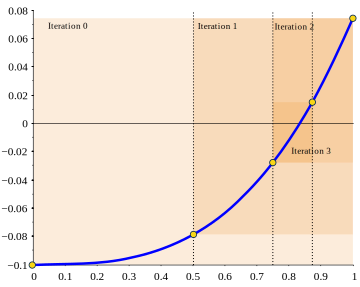
\includegraphics[scale=1]{./figures/f1_tol.pdf}
 \end{center}
 \caption{ \label{fig:fn:tol}
  Illustration of $x$- and $y$-tolerances for bisection iterations}
\end{figure}

\newpage

It takes very little text to fill a page in this format, but there is even less text on most of these sample pages.

\section{Why we are doing it}
It is usually a good idea to give reasons for your research.  If you do not, the people who paid you to waste all that time will feel really bad about it, and then they will not provide the same opportunity to future students.

\newpage

I need this page to see what even-numbered pages look like.

\appendix
% !TEX root = ../thesis-sample.tex
\appendix
\chapter{Methods}
Here is how to implement the methods.

\section{Bisection}
The easiest method.

\begin{equation}\label{eq:sum}
    x_k = \frac{a_k+b_k}{2}
\end{equation}

\section{False Position}
The next one.

\chapter{Using Appendices}    \label{app:appendix}

This section might be referencing code and options that no longer exist in this version of the thesis class.
It should also be updated as well.

This appendix contains the portion of the users' manual that describes
how to use appendices with this template.  It is put in this appendix
rather than in Chapter~\cref{chap:intro} simply so that there are two
appendices, so that a list of appendices can appear earlier in the
document.

\section{Starting the Appendices}
Actually, using appendices is quite simple.  Immediately after the end
of the last chapter and before the start of the first appendix, simply
enter the command \verb|\appendix|.  This will tell \LaTeX~to change
how it interprets the commands \verb|\chapter|, \verb|\section|,
\textit{etc.}

Each appendix is actually a chapter, so once the \verb|\appendix|
command has been called, start a new appendix by simply using the
\verb|\chapter| command.

Note that the \verb|\appendix| command should be called only
once--not before the start of each appendix.



\bibliographystyle{IEEEtran}
\bibliography{thesis-bib}

% appendices must appear after
% !TEX root = ../thesis-sample.tex
\appendix
\chapter{Methods}
Here is how to implement the methods.

\section{Bisection}
The easiest method.

\begin{equation}\label{eq:sum}
    x_k = \frac{a_k+b_k}{2}
\end{equation}

\section{False Position}
The next one.

\chapter{Using Appendices}    \label{app:appendix}

This section might be referencing code and options that no longer exist in this version of the thesis class.
It should also be updated as well.

This appendix contains the portion of the users' manual that describes
how to use appendices with this template.  It is put in this appendix
rather than in Chapter~\cref{chap:intro} simply so that there are two
appendices, so that a list of appendices can appear earlier in the
document.

\section{Starting the Appendices}
Actually, using appendices is quite simple.  Immediately after the end
of the last chapter and before the start of the first appendix, simply
enter the command \verb|\appendix|.  This will tell \LaTeX~to change
how it interprets the commands \verb|\chapter|, \verb|\section|,
\textit{etc.}

Each appendix is actually a chapter, so once the \verb|\appendix|
command has been called, start a new appendix by simply using the
\verb|\chapter| command.

Note that the \verb|\appendix| command should be called only
once--not before the start of each appendix.




\end{document}
